\documentclass[12pt]{report}
\usepackage[utf8]{inputenc}
%\usepackage[T1]{fontenc}
\usepackage{tgbonum}
\usepackage[english]{babel}
\usepackage{graphicx}
\usepackage{amsmath}
\usepackage{amssymb}
\usepackage{hyperref}
\usepackage{epsf}
\usepackage{float}
\usepackage{mathpazo}
\usepackage{pifont}
\usepackage{color}
\definecolor{mygreen}{RGB}{70, 180, 90}
\definecolor{mylilas}{RGB}{255, 117, 45}
\definecolor{cadr}{rgb}{0.89, 0.0, 0.13}
\definecolor{myblue}{RGB}{0, 102, 204}
\usepackage{caption}
\usepackage{subcaption}
\usepackage{subfloat}
\usepackage
[
a4paper,% other options: a3paper, a5paper, etc
left=3cm,
right=3cm,
top=3cm,
bottom=3cm,
]{geometry}
%\geometry{hmargin=3.5cm, vmargin=2.5cm}
\usepackage{fancyhdr}
\pagestyle{fancy}
\fancyhf{}
\rfoot{\thepage}
\renewcommand{\headrulewidth}{0pt}
\usepackage{color}
\graphicspath{{DWGs/}}
\usepackage{graphicx}
\usepackage{wrapfig}
\usepackage{graphicx}
\usepackage{multicol}
\usepackage{enumitem}
\usepackage{xcolor}
\usepackage{framed}
\usepackage{bm}
\definecolor{shadecolor}{RGB}{139, 231, 3}
\usepackage{epigraph}

\usepackage{mathpazo}
\usepackage[framemethod=TikZ]{mdframed}
\usepackage{lipsum}

\usepackage{color}
\definecolor{color-box-border-equation}{RGB}{200,200,200}
\definecolor{color-box-background-equation}{RGB}{250,250,250}

\definecolor{color-box-border-code}{RGB}{54,119,168}
\definecolor{color-box-background-code}{RGB}{236,245,255}

\mdfdefinestyle{equation-frame}{%
    linecolor=color-box-border-equation,
    outerlinewidth=1pt,
    roundcorner=10pt,
    innertopmargin=\baselineskip,
    innerbottommargin=\baselineskip,
    innerrightmargin=20pt,
    innerleftmargin=20pt,
    backgroundcolor=color-box-background-equation}
    
\mdfdefinestyle{exercise-frame}{%
    linecolor=color-box-border-code,
    outerlinewidth=1pt,
    roundcorner=10pt,
    innertopmargin=\baselineskip,
    innerbottommargin=\baselineskip,
    innerrightmargin=20pt,
    innerleftmargin=20pt,
    backgroundcolor=color-box-background-code}

\usepackage{pifont}

\usepackage{tcolorbox}
\definecolor{mycolor}{rgb}{0.122, 0.435, 0.698}

\newtcbox{\mb}{nobeforeafter,colframe=mycolor,colback=mycolor!10!white,boxrule=0.5pt,arc=4pt,
  boxsep=0pt,left=6pt,right=6pt,top=3pt,bottom=3pt,tcbox raise base}

\usepackage{eso-pic}
\newcommand\BackgroundPic{%
\put(-50,-0){%
\parbox[b][\paperheight]{\paperwidth}{%
\vfill
\centering
\includegraphics[height=\paperheight,%
keepaspectratio]{DWGs/cover.png}%
\vfill
}}}

%\usepackage{emerald}
\usepackage[T1]{fontenc}

\usepackage{anyfontsize}
\usepackage{t1enc}
\newcommand{\heart}{\ensuremath\varheartsuit}
\usepackage{tikz}
\usetikzlibrary{positioning}

% CHAPTER STYLE =================================================

\makeatletter
\def\thickhrulefill{\leavevmode \leaders \hrule height 1ex \hfill \kern \z@}
\def\@makechapterhead#1{%
  \vspace*{10\p@}%
  {\parindent \z@ \raggedleft \reset@font
            \scshape \@chapapp{} \thechapter
        \par\nobreak
        \interlinepenalty\@M
    \Huge \bfseries #1\par\nobreak
    %\vspace*{1\p@}%
    %\hrulefill
    \par\nobreak
    \vskip 50\p@
  }}
\def\@makeschapterhead#1{%
  \vspace*{10\p@}%
  {\parindent \z@ \raggedleft \reset@font
            \scshape \vphantom{\@chapapp{} \thechapter}
        \par\nobreak
        \interlinepenalty\@M
    \Huge \bfseries #1\par\nobreak
    %\vspace*{1\p@}%
    %\hrulefill
    \par\nobreak
    \vskip 50\p@
  }}

\begin{document}

% TITLE PAGE ====================================================

\begin{titlepage}
\AddToShipoutPicture*{\BackgroundPic}
\ \\[4cm]
{\sffamily \color{white}
\begin{center}
\fontsize{76}{10}\selectfont \fontfamily{qcr}\selectfont Fluid

\vskip 5\p@

\fontsize{55}{10}\selectfont \fontfamily{qcr}\selectfont Toolbox

\vskip 10\p@

%\fontsize{25}{10} \selectfont \fontfamily{augie}\selectfont with Python

\end{center}
}
\vfill
{\fontsize{20}{20}\color{white}\sffamily \href{https://kamilazdybal.github.io/}{\texttt{kamilazdybal.github.io}} \hfill\color{white} Kamila Zdybał}

{\fontsize{10}{10}\color{white}\sffamily PDFs for explorers and experimenters}
\end{titlepage}


% EX LIBRIS PAGE ================================================

\thispagestyle{empty}
\begin{center}
\vspace*{3cm}
\includegraphics[width = 80mm]{ex_libris_arduino.jpg}

\vspace*{1cm}

{\fontsize{18}{10}\selectfont \fontfamily{pbk}\selectfont E X \,\, L I B R I S $\cdotp$ K A M I L A}

\vspace*{2cm}

Copyright \textcopyright \, K. Zdybał, 2025

For more projects similar to this one

visit my personal website: \verb|kamilazdybal.github.io|

or visit me on GitHub: \verb|@kamilazdybal|

To contact me personally drop me a line at:

\verb|kamilazdybal at gmail dot com|

\vspace*{2cm}

\verb|Fluid Toolbox|

\verb|version 1.0|

Typeset with \ding{170} for \LaTeX

\vspace*{1.8cm}

\noindent This work is licensed under the Creative Commons

Attribution-NonCommercial-ShareAlike 4.0 International 

(CC BY-NC-SA
4.0) license.
\end{center}

\setlength{\parskip}{0.6em}
\setlength{\parindent}{0cm}

\tableofcontents
\chapter*{Preface}
\thispagestyle{empty}
\chaptermark{Preface}
% Fluid Toolbox content

\rightline{{\rm \textit{"Use it well."}}}

\rightline{{\rm --- Prof. Albus Dumbledore}}

\texttt{\textbf{Fluid Toolbox}} is a collection of human-readable, pseudo-random study notes. It contains deeper explanations of various fluid dynamics concepts. It is meant to be used complimentary to the regular textbook since it may provide additional insights but it will not substitute the thoroughness of the standard course in the subject. I believe that working side by side with the course, it can become a useful toolbox of concepts that are ready-to-use and ready-to-understand.

\subsection*{Why is this text created?}

I have a goal of collecting the most important fluid mechanics concept in one place. Much of the knowledge presented here comes from my search for understanding that I was often missing when reading textbooks, and which was difficult to find in a way that would be pleasant, intuitive and make sense to me. Some of the understanding presented here comes from my personal explorations and thinking on the subject. I have hopes that it will become a helpful resource that you have been looking for. I would also like to challenge you to ponder more deeply about the concepts presented here and to seek the beauty of fluid mechanics.

\subsection*{Code of conduct}
\thispagestyle{empty}
There are a few things that I would like to state at the very beginning to give you an honest overview of what you will encounter later in this text.

\begin{enumerate}
\item I want to take you through the journey of learning as you read these notes. Above all, I will know that it was worth writing this document if you enjoyed the journey or reading it and learning from it.
\item It's not enough to read a textbook or watch a lecture. The real learning and understanding comes when it's only you, your head and a blank piece of paper. Reading a textbook is an easy task to do, so is watching a lecture. When you become a spectator, it's an easy trap  fooling yourself that you understood something. It's when you have a chance to take action in your learning that you can really test your knowledge and deep understanding.
\item I believe in the quote by Richard Feynman: \textit{Study hard what interest you the most in the most undisciplined, irreverent and original manner possible.} I will sometimes ask a brain-teasing question or challenge you to \textit{pause and ponder}. But also do challenge yourself and don't let your imagination be limited by simply following the pages of any textbook!
\item Programming is a great way to roll your sleeves and put things into action.
\item This document will be alive for quite some time. I will be coming back to it to add or improve things. You can always access the newest version through my GitHub site:

\verb|https://kamilazdybal.github.io|
\end{enumerate}

\,\,

Please feel free to contact me with any suggestions, corrections, or comments: \verb|kamilazdybal at gmail dot com|.


\newpage
\chapter*{Acknowledgements}
\thispagestyle{empty}
\chaptermark{Ack}

{\fontsize{12}{12}\rightline{\textit{I am grateful to all people I encountered in my life}}}

\vspace*{0.5cm}

{\fontsize{12}{12}\rightline{\textit{who supported my passion for studying fluid motion.}}}

\vspace*{0.5cm}

{\fontsize{12}{12}\rightline{\textit{Among the first ones were Y. Çengel and J. Cimbala}}}

\vspace*{0.5cm}

{\fontsize{12}{12}\rightline{\textit{in their inspiring fluid mechanics textbook.}}}

\vspace*{2cm}
\rightline{{\rm \textit{Zürich, Switzerland, 2025}}}


\newpage

% - - - - - - - - - - - - - - - - - - - - - - - - - - - - - - - - - - - - - - - - - - - - - - - - 
\chapter{Changes} \label{chap:changes}

%\rightline{{\rm \textit{Ch-ch-ch-ch-changes}}}
\rightline{{\rm \textit{Turn and face the strange}}}
\rightline{{\rm \textit{Ch-ch-changes}}}
\rightline{{\rm \textit{There's gonna have to be a different man}}}

\rightline{{\rm --- David Bowie}}


Changes are modeled by derivatives. Derivative explains how much one variable $\phi_1$ changes when we change the other $\phi_2$, and we express this in mathematical terms:

\begin{equation}\label{eq:change-d}
\frac{d \phi_1}{d \phi_2}
\end{equation}

where the letter $d$ stands for \textit{the change of...} and is later followed by the variable that we are speaking of. So really the above ratio means: there is this much change of variable $\phi_1$ per this much change of variable $\phi_2$. In fluid dynamics, you will find that we are most interested with two types of changes: change in time and change in space (position). Therefore you will most often encounter $dt$ or $dx$, $dy$, $dz$ in the denominator of various forms of Eq.~(\ref{eq:change-d}). Since we live in the three-dimensional space with a time arrow, it is justifiable why these two have the biggest popularity, right?

There is also another mathematical expression for a derivative and it is:

\begin{equation}\label{eq:change-partial}
\frac{\partial \phi_1}{\partial \phi_2}
\end{equation}

The operator $\partial$ (called ''partial`` or ''del``) also stands for \textit{the change of...} but it also gives you a hint that the variable $\phi_1$ can change with the change of variables other than $\phi_2$. Perhaps it can also change with some $\phi_3$ and $\phi_4$, even though in this particular ratio from Eq. (\ref{eq:change-partial}) we are only interested in the change with respect to $\phi_2$.

\section{What does it mean for a quantity to change in time and in space?}


\subsection{Steady-state case and a time derivative}

\section{Convention for the sign of a derivative}

For the purpose of this demonstration we will look at the derivative $\frac{dp}{dx}$ -- change in pressure per change in the $x$-axis position -- which is often encountered in fluid dynamics. We will lay the ground for what does it mean for this derivative to be positive, negative or zero, and why the reasoning makes sense.

Suppose that the initial point is marked with \textcolor{myblue}{$(i)$} and it is always a point at coordinate $x$. The point to which we move after one space-step, the final point, is marked with \textcolor{myblue}{$(f)$} and is either at $x+dx$ or $x - dx$ coordinate, depending on the positive or negative change that we decide to make. The direction of the change on the $x$-axis is marked with a blue arrow.

\begin{figure}[H]
\begin{subfigure}[t]{.46\textwidth}
\centering
\includegraphics[scale=1]{dp-dx-pos-neg.pdf}
\caption{$\frac{dp}{dx} > 0$ with positive change in $x$.}
\end{subfigure}
\begin{minipage}[t]{.07\textwidth}
$ $
\vspace*{1.5cm}
\end{minipage}
\begin{subfigure}[t]{.46\textwidth}
\centering
\includegraphics[scale=1]{dp-dx-neg-neg.pdf}
\caption{$\frac{dp}{dx} > 0$ with negative change in $x$.}
\end{subfigure}
\begin{subfigure}[t]{.46\textwidth}
\centering
\includegraphics[scale=1]{dp-dx-pos-pos.pdf}
\caption{$\frac{dp}{dx} < 0$ with positive change in $x$.}
\end{subfigure}
\begin{minipage}[t]{.08\textwidth}
$ $
\end{minipage}
\begin{subfigure}[t]{.46\textwidth}
\centering
\includegraphics[scale=1]{dp-dx-neg-pos.pdf}
\caption{$\frac{dp}{dx} < 0$ with negative change in $x$.}
\end{subfigure}
\caption{Sign of the $\frac{dp}{dx}$ derivative versus directions of change along the $x$-axis.}
\label{fig:dp-dx-signs}
\end{figure}

We will now find out for all cases which pressure, at \textcolor{myblue}{$(i)$} or at \textcolor{myblue}{$(f)$} must be larger. Our aim is to show that situations (a) and (b) in Figure \ref{fig:dp-dx-signs} must be equivalent -- they explain the same physical phenomena. In both of these cases we will show that the pressure is increasing with the increasing $x$-coordinate, independent of whether we decide to take a step to the right or to the left of our initial point \textcolor{myblue}{$(i)$}. 

We will show the analogical result can be said about situations (c) and (d) but in this case the pressure is decreasing with the increasing $x$-coordinate.



\subsection{Closing note}

The analysis done in this section is often necessary in order to find out whether or not to ''put a minus sign`` in front of expressions. For instance, as we will show later in the text, such reasoning can help us understand why there is a minus sign in the Euler equation for a fluid element experiencing pressure force: $dp = - \rho \upsilon d \upsilon$. Oftentimes, the sign of a derivative tells an important information about the nature of the physical phenomena.







% - - - - - - - - - - - - - - - - - - - - - - - - - - - - - - - - - - - - - - - - - - - - - - - - 
\chapter{Differentiation}

%Differentiation is a way to make discrete things continuous.

% - - - - - - - - - - - - - - - - - - - - - - - - - - - - - - - - - - - - - - - - - - - - - - - - 
\chapter{Material derivative}

\section{Where space, time, and fluid flow meet}

The material derivative describes the \textit{total experienced} change in quantity $\bullet$ as \textit{time goes on} \textbf{and} as we \textit{move} across the field of $\bullet$ with fluid velocity, $\vec{\bm{V}} = \langle u, \upsilon, w \rangle$. Hence, the material derivative requires two ingredients; these are visualized in Fig.~\ref{fig:material-derivative-two-ingredients}. The first ingredient is the field of $\bullet$, which can change spatially and temporally (Fig.~\ref{fig:material-derivative-two-ingredients}a). The second ingredient is the associated fluid velocity field, $\vec{\bm{V}}$ (Fig.~\ref{fig:material-derivative-two-ingredients}b). In this chapter, you can substitute for $\bullet$ any interesting physical quantity that you'd like, such as density, $\rho$, or temperature, $T$. Interestingly, this quantity does not need to be a scalar, but can also be a vector or even a tensor.
\begin{figure}[H]
\centering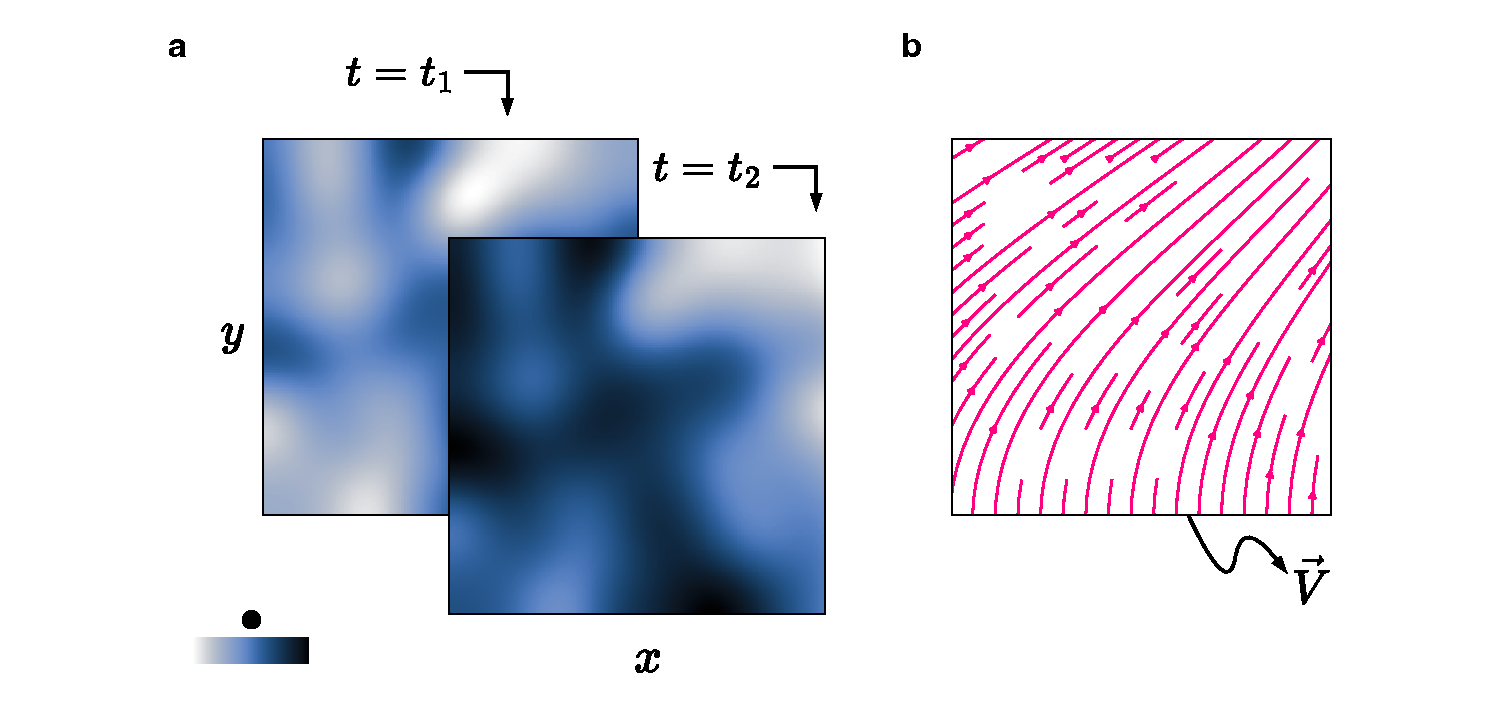
\includegraphics[width=15cm]{material-derivative-two-ingredients.pdf}
\caption{Two ingredients needed to compute the material derivative: (\textbf{a}) the field of $\bullet$, which can change spatially and temporally, and (\textbf{b}) the associated fluid velocity field, $\vec{\bm{V}}$.}
\label{fig:material-derivative-two-ingredients}
\end{figure}

To first start thinking about the material derivative visually, you may consider a 2D field of $\bullet$ that changes in time and space, just like the one presented in Fig.~\ref{fig:material-derivative-two-ingredients}a. In Fig.~\ref{fig:material-derivative-example}, let's look at the possible reasons for why we might experience change in $\bullet$. In the absence of spatial movement over the $(x,y)$ grid we can only experience change in $\bullet$ if $\bullet$ varies in time. Similarly, in the absence of temporal variation in $\bullet$, we can experience change in $\bullet$ only if we travel along the $(x,y)$ grid and $\bullet$ varies over that grid. With both time and motion present, we experience a superposition of these two effects. That will be our total experienced change in $\bullet$. I will emphasize, however, that in the definition of the material derivative our movement is restricted to one defined by the fluid flow. Hence, we specifically use the flow velocity, $\vec{\bm{V}}$, and not any other velocity\footnote{That said, one could, potentially, define a generalization of the material derivative to allow for an arbitrary velocity! Such a new quantity will have a different physical meaning though.}.
\begin{figure}[H]
\centering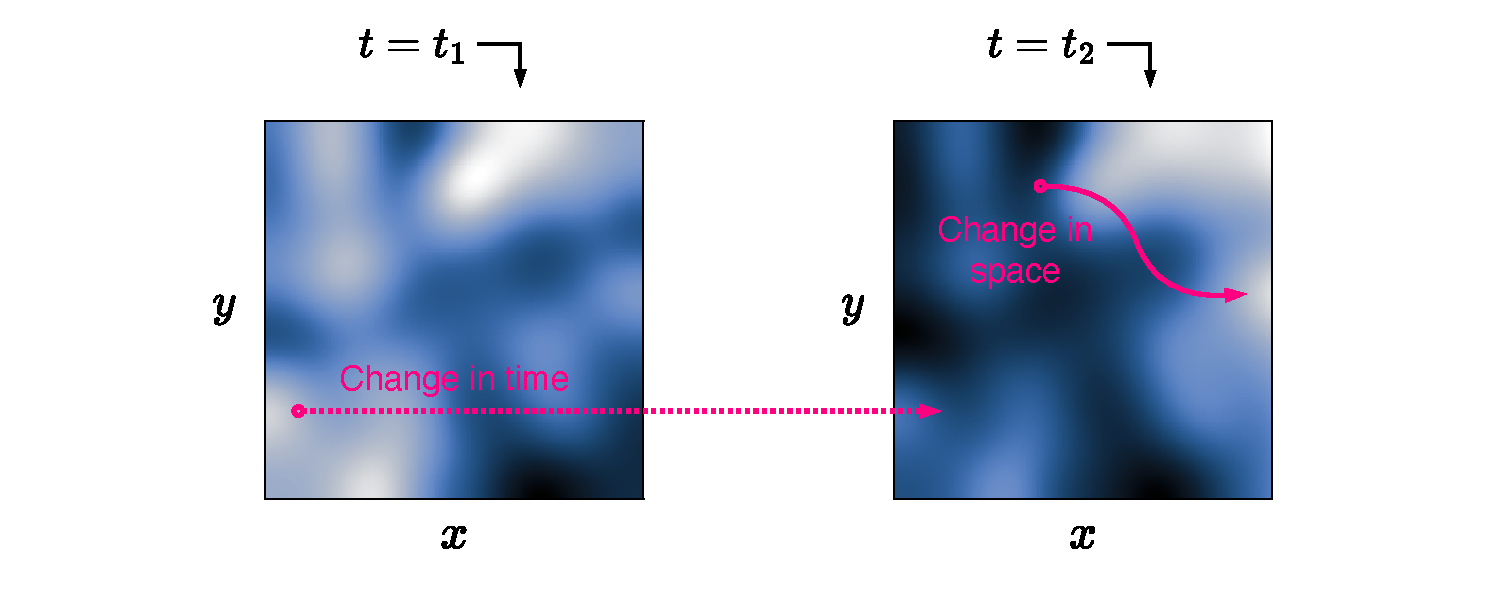
\includegraphics[width=15cm]{material-derivative.pdf}
\caption{A 2D field of some scalar quantity, $\bullet$, that changes in time, $t$, and space, $(x, y)$. We also consider the associated fluid velocity field, $\vec{\bm{V}}$. The material derivative is a superposition of two reasons for why $\bullet$ can change.}			
\label{fig:material-derivative-example}
\end{figure}

In mathematical terms, the material derivative, $\frac{D}{Dt}$, is an operator acting on $\bullet$ such that
\begin{equation} \label{eq:material-derivative}
\frac{D \bullet}{D t} \equiv \frac{\partial \bullet}{\partial t} + \vec{\bm{V}} \cdot \nabla \bullet \, .
\end{equation}
The superposition that I mentioned before is embedded in the two terms on the right-hand-side of Eq.~(\ref{eq:material-derivative}). We can now dissect these two terms to better understand why introducing the material derivative is very useful when studying fluid motion.

First, we have $\frac{\partial \bullet}{\partial t}$ which is the plain old\footnote{See Chapter~\ref{chap:changes}.} partial derivative of $\bullet$ with respect to time. It says that at all possible locations in space, and at any one location, the quantity $\bullet$ can evolve in time. One example of such quantity is temperature. Even if we remain stationary in a specific location, say in a corner of a room, we can still experience change in temperature because our room might be heated (or cooled) and the temperature in our little corner changes in time because of that. The term $\frac{\partial \bullet}{\partial t}$ gives us a recipe for \textit{how} that temperature changes in time in every location of the room.

Second, we have $\vec{\bm{V}} \cdot \nabla \bullet$, that is, a gradient vector, $\nabla \bullet = \langle \frac{\partial \bullet}{\partial x}, \frac{\partial \bullet}{\partial y}, \frac{\partial \bullet}{\partial z} \rangle$, dotted with the fluid velocity vector, $\vec{\bm{V}}$. 
%At this point, you might remind yourself of the intuition behind taking a dot product between two vectors from Fig.~\ref{fig:circulation-dot-product}. 
The gradient of $\bullet$ is a vector field that describes directions in which $\bullet$ varies. If, and only if, your own movement is aligned (at least to some extent) with the direction of $\bullet$'s gradient, you will experience a change in quantity $\bullet$. Otherwise, if you walk along an isocurve of $\bullet$, you will not experience any change in $\bullet$. The dot product taken between $\vec{\bm{V}}$ and $\nabla \bullet$ measures the degree of that alignment.

In other words, the first term on the right-hand-side of Eq.~(\ref{eq:material-derivative}) describes how we will experience change in $\bullet$ in the absence of our motion through the field of $\bullet$. The second term describes how we will experience additional change in $\bullet$ due to moving around through the field of $\bullet$ but with a very specific velocity, $\vec{\bm{V}}$. The material derivative is a neat superposition of these two factors for why $\bullet$ can change. It is also a shorthand for describing change in $\bullet$ in a moving fluid and it has been created because this superposition of effects frequently appears in the governing equations of fluid dynamics. Writing it in short as $\frac{D}{D t}$ simply makes our life easier.

\begin{mdframed}[style=exercise-frame]

\subsection*{Hungry for more?}

You can find a great intuitive description of a material derivative in Chapter~3, \S3.5 of the \textit{Transport Phenomena} textbook by Bird, Stewart \& Lightfoot \cite{bird2002transport}. They delineate differences between various derivatives on the example of following fish in a river.

\end{mdframed}

%You might rightfully ask: How is the material derivative different from the regular derivative, say $\frac{d}{dt}$ or $\frac{\partial}{\partial t}$? Well, it's simply a special sum of those regular derivatives, such that it accounts for change in time and movement through space \textit{simultaneously}. Therefore, its practical computation isn't mathematically any different from computing regular partial derivatives. 

Finally, I would like to present two more ways of writing Eq.~(\ref{eq:material-derivative}) just to expose you to other possible notations that you might encounter in textbooks. 
In the most general 3D case, where $\vec{\bm{V}} = \langle u, \upsilon, w \rangle$, we can expand the dot product terms to obtain:
\begin{equation} \label{eq:material-derivative-full}
\frac{D \bullet}{D t} \equiv \frac{\partial \bullet}{\partial t} + u \frac{\partial \bullet}{\partial x} + \upsilon \frac{\partial \bullet}{\partial y} + w \frac{\partial \bullet}{\partial z} \, .
\end{equation}
A yet another way of writing the equation above that you might sometimes encounter is the following:
\begin{equation} \label{eq:material-derivative-ein stein}
\frac{D \bullet}{D t} \equiv \frac{\partial \bullet}{\partial t} + V_i \frac{\partial \bullet}{\partial i} \, .
\end{equation}
This way of writing Eq.~(\ref{eq:material-derivative-full}) is using the Einstein notation where it is implied that you should substitute for the dummy index $i$ every possible spatial dimension, \textit{i.e.}, $x$, $y$, and $z$, and, as you substitute, you also sum up all the terms that form for each possible $i$.

\section{Pause and ponder}

Let's look at some alternative ways to describe change in both space and time and see why they wouldn't be equally useful as Eq.~(\ref{eq:material-derivative})! Suppose I present you with the following quantity:
\begin{equation} \label{eq:all-derivatives}
\frac{\partial \bullet}{\partial t} + \frac{\partial \bullet}{\partial x} + \frac{\partial \bullet}{\partial y} + \frac{\partial \bullet}{\partial z} \, .
\end{equation}
How is that quantity different from the definition of the material derivative? In other words, what does the dot product with the velocity vector change in how we described change in space in Eq.~(\ref{eq:material-derivative-full})?

The velocity vector is not our independent motion through the field of $\bullet$. It is our motion when carried by the fluid flow.


This discussion tells us something deeper about the philosophy of describing fluid motion. Material derivative is inherently tied to the continuum assumption in fluid dynamics.

In essence, the material derivative describes our experience change in $\bullet$ because of our motion with the fluid velocity, even though the change in $\bullet$ might happen precisely \textit{due to} fluid motion, or at least be some function of it. Think about the fluid density, $\rho$, which can change due to local movement of fluid from one location to the next.





% - - - - - - - - - - - - - - - - - - - - - - - - - - - - - - - - - - - - - - - - - - - - - - - - 
\chapter{Divergence theorems}

%Differentiation is a way to make discrete things continuous.

% - - - - - - - - - - - - - - - - - - - - - - - - - - - - - - - - - - - - - - - - - - - - - - - - 
\chapter{Common flow types}

%\input{common_flow_types/common_flow_types.tex}

% - - - - - - - - - - - - - - - - - - - - - - - - - - - - - - - - - - - - - - - - - - - - - - - - 
\chapter{Drag force}

%\input{drag_force/drag_force.tex}

% - - - - - - - - - - - - - - - - - - - - - - - - - - - - - - - - - - - - - - - - - - - - - - - - 
\chapter{Circulation}

%

Circulation is defined as:

\begin{equation}
\Gamma = \oint_C \vec{\upsilon} \cdot \vec{dl}
\end{equation}

The dot product, $\vec{\upsilon} \cdot \vec{dl}$, returns a scalar which is expressing ''how much`` in the direction of the other vector is this vector.

\begin{figure}[H]
\centering\includegraphics[width=5cm]{circulation_dot_prod}
\caption{Dot product of two vectors.}			
\label{fig:circulation-dot-product}
\end{figure}

When they are $\perp$, the dot product is zero.

In the concept of circulation, we ask ''how much`` at any point on the curve $C$ the velocity vector at that point is in the direction of the curve's geometry. Now, that doesn't yet sound as something to do with ''circulating``. For the moment, I would think that it's more of an ''on-trackness``. Something, that in real world would be for instance the measure of how much the vehicle's velocity is in the direction of the road geometry (and we would hope that's  .

But to start 
, notice an important detail of ''$\circ$`` on the integral symbol, which signals that the curve should be a closed curve -- a loop -- although not necessarily a perfect circle.

When you perform integration, which means summing up every little $\vec{\upsilon} \cdot \vec{dl}$ as you go around the loop, you count ''how much`` at every point on the loop, the velocity vector at these points is in the direction of the loop's geometry (at these points).

If we were to place a small particle at some starting point $P$ on the loop, the circulation would tell us ''how much`` the velocity field which this particle is subjected to, is tending to move that particle around the loop.

It can be very intuitive when you take a look at these two pictures:





It's no surprise that when the velocity is everywhere perpendicular to the loop's geometry, the circulation around the loop is zero. If you were to place a particle at any point on the loop, such velocity field would act to immediately displace the particle off the loop. Therefore, the particle would have no way of ''circulating`` around the loop.

On the other extreme is the case when the velocity field is everywhere tangent to the loop's geometry. Anywhere the particle goes on the loop, the velocity at that point would act to keep the particle moving around the loop.

Questions:

\begin{enumerate}
\item Why closed loop? Would it have any meaning if we calculated circulation along any general spline?

\item How to chose loops so that the circulation we calculate is of the most meaning to us?

\item What does the zero, positive, negative circulation mean?

\item Can circulation be infinite?

\item For what velocity field, $\vec{\upsilon}$, and the corresponding loop, $C$, is circulation zero?
\end{enumerate}



% - - - - - - - - - - - - - - - - - - - - - - - - - - - - - - - - - - - - - - - - - - - - - - - - 
\chapter{Vorticity}

%\input{vorticity/vorticity.tex}

% - - - - - - - - - - - - - - - - - - - - - - - - - - - - - - - - - - - - - - - - - - - - - - - - 
\chapter{Stoke's theorem}

%\input{stokes_theorem/stokes_theorem.tex}

% - - - - - - - - - - - - - - - - - - - - - - - - - - - - - - - - - - - - - - - - - - - - - - - - 
\chapter{Nondimensionalizing}

%\input{nondimensionalizing/nondimensionalizing.tex}

% - - - - - - - - - - - - - - - - - - - - - - - - - - - - - - - - - - - - - - - - - - - - - - - - 
\chapter{Conservation of mass}

%In this chapter we present the derivation of the conservation of mass equation, otherwise known as the \textbf{continuity equation}. In principle, it states that mass cannot be lost nor created.

We begin by writing out the overall mass balance inside any control volume CV. The net change of mass inside the control volume is equal to the mass flowing into the CV minus the mass flowing out of the CV. Note here, that when the net change of mass in a CV is not zero (unsteady case), it can only be due to either compression (more mass flowing in than flowing out) or decompression (more mass flowing out than flowing in). The general mass balance is:

\begin{equation} \label{eq:net_change}
\text{net change} = \text{flow in} - \text{flow out}
\end{equation}

\section{Mass flow rate}

\section{Derivation using control volume}

We are going to write out the RHS of the equation \ref{eq:net_change} as the difference between mass flow rate in and mass flow rate out in three Cartesian directions.

In the $x$-direction:

\begin{equation}
\Big( \rho u - \frac{\partial (\rho u)}{\partial x} \frac{dx}{2} \Big) dy dz - \Big( \rho u + \frac{\partial (\rho u)}{\partial x} \frac{dx}{2} \Big) dy dz = - \frac{\partial (\rho u)}{\partial x} dx dy dz
\end{equation}

In the $y$-direction:

\begin{equation}
\Big( \rho v - \frac{\partial (\rho v)}{\partial y} \frac{dy}{2} \Big) dx dz - \Big( \rho v + \frac{\partial (\rho v)}{\partial y} \frac{dy}{2} \Big) dx dz = - \frac{\partial (\rho v)}{\partial y} dy dx dz
\end{equation}

In the $z$-direction:

\begin{equation}
\Big( \rho w - \frac{\partial (\rho w)}{\partial z} \frac{dz}{2} \Big) dx dy - \Big( \rho w + \frac{\partial (\rho w)}{\partial z} \frac{dz}{2} \Big) dx dy = - \frac{\partial (\rho w)}{\partial z} dz dx dy
\end{equation}

The net change in time of mass can be written as:

\begin{equation}
\frac{\partial \rho}{dt} dx dy dz
\end{equation}

Putting all the terms together into equation \ref{eq:net_change} we obtain:

\begin{equation}
\frac{\partial \rho}{dt} dx dy dz = - \frac{\partial (\rho u)}{\partial x} dx dy dz - \frac{\partial (\rho v)}{\partial y} dy dx dz - \frac{\partial (\rho w)}{\partial z} dz dx dy
\end{equation}

Dividing both sides by $dx dy dz$ we get:

\begin{equation} \label{eq:continuity_general}
\frac{\partial \rho}{dt} = - \frac{\partial (\rho u)}{\partial x} - \frac{\partial (\rho v)}{\partial y} - \frac{\partial (\rho w)}{\partial z}
\end{equation}

Lastly, we can observe that the divergence of the quantity $\rho \vec{V}$ is:

\begin{equation}
\nabla (\rho \vec{V}) = \nabla (\rho \langle u, v, w \rangle) = \nabla \langle \rho u, \rho v, \rho w \rangle = \frac{\partial (\rho u)}{\partial x} + \frac{\partial (\rho v)}{\partial y} + \frac{\partial (\rho w)}{\partial z}
\end{equation}

So in the end, we can further write the RHS of the equation \ref{eq:continuity_general} in a shorter format as:

\begin{equation} \label{eq:continuity_divergence}
\frac{\partial \rho}{dt} = - \nabla \cdot (\rho \vec{V})
\end{equation}

\section{Special cases of density function}

In the most general case, the density $\rho$ is a function of time and space $\rho = \rho(t, x, y, z)$ and the equation \ref{eq:continuity_divergence} is written out for the most general case. Special cases can be defined when certain restrictions are imposed on the density function.

\subsection{Incompressible flow}

When we assume that the density is constant in space, it can be taken out front of the divergence operator and the incompressible continuity equation is:

\begin{equation} \label{eq:continuity_incompressible}
\frac{\partial \rho}{dt} = - \rho \nabla \cdot \vec{V}
\end{equation}

The above equation corresponds to the density that is constant throughout the flow field at any moment in time, but can change in time in the entire flow field.




\subsection{Incompressible, steady flow}

The steady flow can be further combined with the incompressible condition, which disables the density to change both in time and space. The stead-state incompressible continuity equation then becomes:

\begin{equation} \label{eq:continuity_stst_incompressible}
0 = \nabla \cdot \vec{V}
\end{equation}

or writing the above equation with the use of partial differentiation operator:

\begin{equation}
\frac{\partial u}{\partial x} + \frac{\partial v}{\partial y} + \frac{\partial w}{\partial z} = 0
\end{equation}


\subsection{Compressible, steady flow}

First, when the density $\rho$ is only a function of position $\rho = \rho(x,y,z)$ and does not change in time at any point in the flow field, we arrive at the steady state condition where the derivative $\frac{\partial \rho}{dt} = 0$.

The continuity equation then becomes:

\begin{equation} \label{eq:continuity_stst}
0 = - \nabla \cdot (\rho  \vec{V})
\end{equation}



\section{Dimension reduction}




\section{Divergence theorem and a different way of looking at the conservation of mass}

% - - - - - - - - - - - - - - - - - - - - - - - - - - - - - - - - - - - - - - - - - - - - - - - - 
\chapter{Gauss's law}

%Differentiation is a way to make discrete things continuous.

% - - - - - - - - - - - - - - - - - - - - - - - - - - - - - - - - - - - - - - - - - - - - - - - - 
\chapter{Reynolds number}

%\input{reynolds_number/reynolds_number.tex}

% - - - - - - - - - - - - - - - - - - - - - - - - - - - - - - - - - - - - - - - - - - - - - - - - 
\chapter{Constitutive equations}

%\input{constitutive_equations/const_eq.tex}

% - - - - - - - - - - - - - - - - - - - - - - - - - - - - - - - - - - - - - - - - - - - - - - - - 
\chapter{The Navier-Stokes equations}

%\input{navier_stokes/navier_stokes.tex}

% - - - - - - - - - - - - - - - - - - - - - - - - - - - - - - - - - - - - - - - - - - - - - - - - 




\chapter*{Appendix}

\newpage
\thispagestyle{empty}

\chapter*{Ending remarks}



\begin{flushright}

%\ \\[6cm]

\includegraphics[width = 100mm]{cover.png}

\setlength{\parskip}{0.1em}
\setlength{\parindent}{0cm}
\ \\[0.5cm]
\textit{The cover photo:}  

View from the coast of Cres island, Croatia, October 2016.
\ \\[0.1cm]
Photo by: J. Aleksanderek $\copyright$
\end{flushright}



\bibliographystyle{apalike}
\bibliography{bibliography}


\end{document}